\documentclass{article}
\usepackage{tikz}
\usetikzlibrary{positioning}

\begin{document}

\begin{figure}[h]
    \centering
    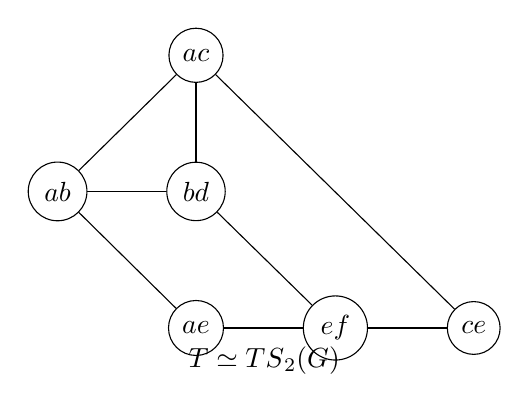
\begin{tikzpicture}[node distance=1cm, auto]
        % Define nodes
        \node (a) [circle, draw] {$ab$};
        \node (b) [circle, draw, right=of a] {$bd$};
        \node (c) [circle, draw, above=of b] {$ac$};
        \node (d) [circle, draw, below=of b] {$ae$};
        \node (e) [circle, draw, right=of d] {$ef$};
        \node (f) [circle, draw, right=of e] {$ce$};

        % Draw edges
        \draw (a) -- (b);
        \draw (a) -- (c);
        \draw (a) -- (d);
        \draw (b) -- (c);
        \draw (b) -- (e);
        \draw (d) -- (e);
        \draw (e) -- (f);
        \draw (f) -- (c);

        \node at (current bounding box.south) {$T \simeq \text{TS}_2(G)$};
    \end{tikzpicture}
    \hspace{2cm}
    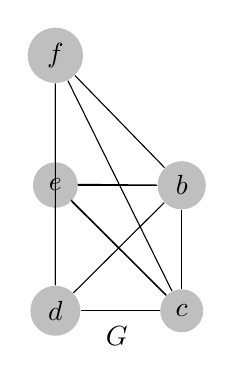
\begin{tikzpicture}[node distance=1cm, auto]
        % Define nodes
        \node (a) [circle, fill=gray!50] {$a$};
        \node (b) [circle, fill=gray!50, right=of a] {$b$};
        \node (c) [circle, fill=gray!50, below=of b] {$c$};
        \node (d) [circle, fill=gray!50, left=of c] {$d$};
        \node (e) [circle, fill=gray!50, above=of d] {$e$};
        \node (f) [circle, fill=gray!50, above=of a] {$f$};

        % Draw edges
        \draw (a) -- (b);
        \draw (a) -- (c);
        \draw (a) -- (d);
        \draw (a) -- (e);
        \draw (a) -- (f);
        \draw (b) -- (c);
        \draw (b) -- (d);
        \draw (b) -- (e);
        \draw (b) -- (f);
        \draw (c) -- (d);
        \draw (c) -- (e);
        \draw (c) -- (f);
        \draw (d) -- (e);
        \draw (d) -- (f);
        \draw (e) -- (f);

        \node at (current bounding box.south) {$G$};
    \end{tikzpicture}
\end{figure}

\end{document}